\documentclass[../ManualeUtente.tex]{subfiles}
\begin{document}
	\section{Guida all'utilizzo}
		Di seguito è presentata una guida all'utilizzo di \progetto.\\
		I termini evidenziati in \textit{\textbf{questo modo}} corrispondono a pulsanti presenti all'interno
		dell'applicazione.
		\subsection{Interfaccia grafica}
			All'avvio dell'applicazione viene presentato il diagramma dei package vuoto (Figura \ref{fig:StartScreen}). Da qui è possibile iniziare immediatamente a sviluppare un nuovo progetto.\\
			L'interfaccia grafica è quindi generalmente composta dalle seguenti componenti:
			\begin{enumerate}
				\item \underline{Menù dell'applicazione} dal quale è possibile interagire con il progetto corrente e con
				le funzionalità offerte dal sistema;
				\item \underline{Area di lavoro} dove è possibile visualizzare e sviluppare i diagrammi: è possibile
				spostarsi all'interno dell'area di lavoro cliccando su uno spazio vuoto e trascinando il mouse
				verso la direzione desiderata. Inoltre è possibile ingrandire e rimpicciolire il contenuto
				del diagramma girando la ruota del mouse;
				\item \underline{Menù degli strumenti} (o toolbar) dal quale è possibile aggiungere elementi al diagramma
				correntemente visualizzato (si aggiorna dinamicamente al cambiare del tipo di diagramma);
				\item \underline{Pannello delle proprietà} che offre tutte le informazioni di un elemento del diagramma
				e la possibilità di modificarle;
				\item \underline{Percorso attuale} che visualizza la posizione corrente (il tipo di diagramma) tra i
				diagrammi del progetto.
			\end{enumerate}
			\begin{figure} [h!]
				\centering
				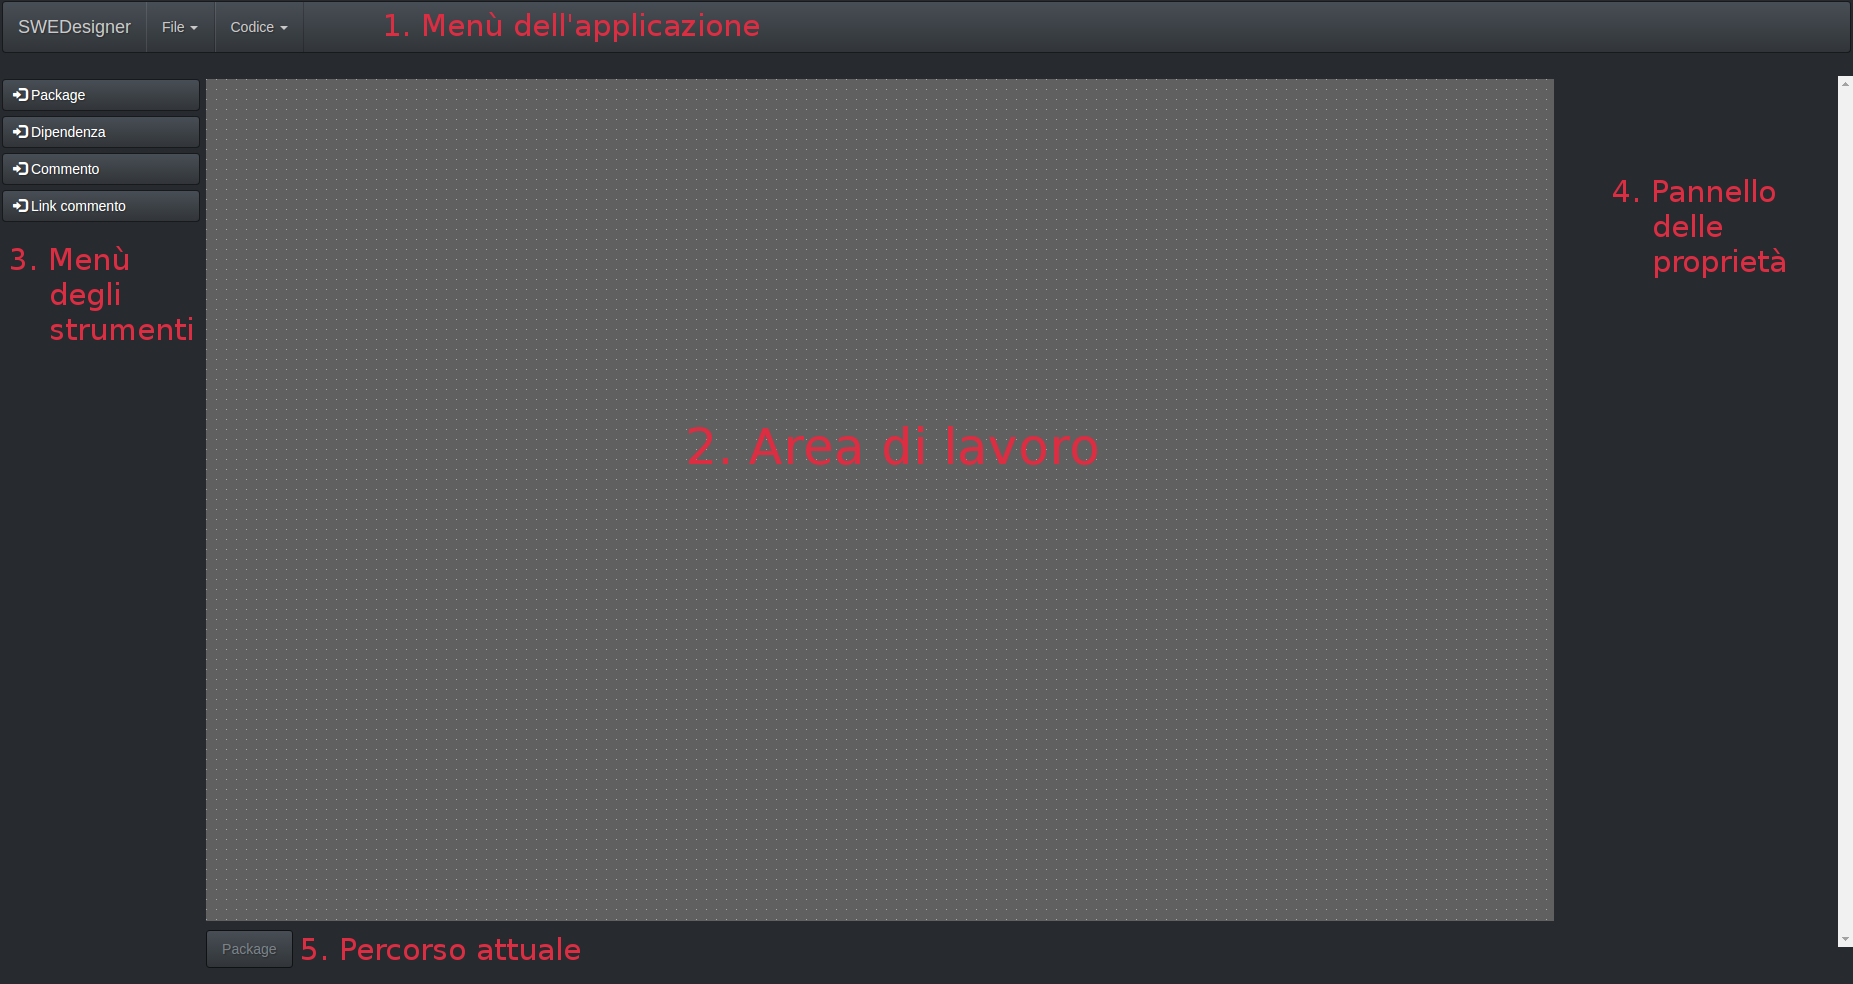
\includegraphics[scale=0.24]{./Immagini/StartScreen.png}
				\caption{Interfaccia grafica - Schermata iniziale}\label{fig:StartScreen}
			\end{figure}
			\subsubsection{Menù dell'applicazione}
				Dal menù dell'applicazione è possibile selezionare le seguenti voci:
				\begin{itemize}
					\item \textit{\textbf{File}}
					\begin{itemize}
						\item \textit{\textbf{Nuovo Progetto}}: elimina il contenuto dell'eventuale progetto
						correntemente aperto ripulendo l'area di lavoro;
						\item \textit{\textbf{Apri}}: apre una finestra di dialogo per poter caricare un
						file di progetto salvato localmente nel proprio pc avente estensione ``.swed'';
						\item \textit{\textbf{Salva}}: salva il progetto correntemente aperto ed esegue il
						download in locale del relativo file con estensione ``.swed'';
						\item \textit{\textbf{Salva con nome}}: salva il progetto correntemente aperto, apre
						una finestra di dialogo per scegliere il nome da dare al file di progetto e ne esegue
						il download in locale.
					\end{itemize}
					\newpage
					\item \textit{\textbf{Codice}}
					\begin{itemize}
						\item \textit{\textbf{Genera Codice Java}}: invia una richiesta al server per generare
						il codice in linguaggio Java del progetto corrente e successivamente avvia il
						download del file compresso ``.zip'' contenente il/i file sorgente/i;
						\item \textit{\textbf{Genera Codice Javascript}}: invia una richiesta al server per
						generare il codice in linguaggio Javascript del progetto corrente e successivamente
						avvia il download del file compresso ``.zip'' contenente il/i file sorgente/i.
					\end{itemize}
				\end{itemize}
			\subsubsection{Percorso attuale}
				Il percorso attuale, sempre visibile in basso a sinistra dell'applicazione, visualizza la
				posizione corrente (il tipo di diagramma) tra i diagrammi del progetto.\\
				Da qui è possibile spostarsi verso un diagramma
				antecedente a quello attuale cliccandone il corrispondente link.
				\begin{figure} [h!]
					\centering
					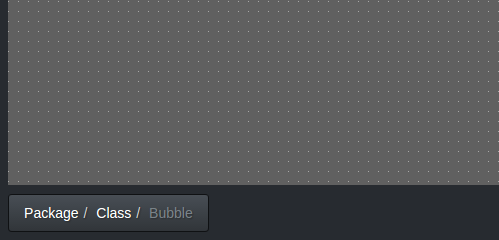
\includegraphics[scale=0.4]{./Immagini/Path.png}
					\caption{Interfaccia grafica - Percorso attuale}\label{fig:Path}
				\end{figure}
		\newpage
		\subsection{Editor del diagramma dei package}
			Nel diagramma dei package è possibile gestire l'architettura al più alto livello disponibile.
			\subsubsection{Menù degli strumenti}
				Sono messi a disposizione i seguenti strumenti per editare il diagramma dei package:
				\begin{itemize}
					\item \textit{\textbf{Package}}: cliccare il pulsante e poi cliccare il luogo desiderato
					dell'area di lavoro per crearvi un package;
					\item \textit{\textbf{Dipendenza}}: cliccare il pulsante, cliccare il package sorgente
					(dipendente) e successivamente quello destinatario per creare una relazione di dipendenza;
					\item \textit{\textbf{Commento}}: cliccare il pulsante e poi cliccare il luogo desiderato
					dell'area di lavoro per crearvi un commento;
					\item \textit{\textbf{Link commento}}: cliccare il pulsante, cliccare il package ed il
					commento desiderati per collegarli.
				\end{itemize}
				Per spostare un elemento (Package o Commento) all'interno dell'area di lavoro, cliccarlo con
				il mouse e trascinarlo verso la posizione desiderata.\\
				Per cambiare un membro di una relazione, trascinarne un apice sull'elemento
				desiderato.\\
				Per spezzare una relazione in un punto specifico della linea, eseguire un doppio click sulla
				posizione desiderata.\\
				Per eliminare un elemento dal diagramma, cliccare sulla rispettiva icona nell'area di lavoro
				avente una croce rossa.
			\subsubsection{Pannello delle proprietà}
				Cliccando su un elemento del diagramma dei package verrà visualizzato il corrispondente pannello
				di dettaglio contenente tutte le proprietà modificabili dell'elemento stesso.\\
				Per modificare una proprietà testuale, editare il campo di testo e successivamente premere il
				tasto "Invio" della tastiera oppure cliccare altrove nell'applicazione.\\
				Per modificare una proprietà non testuale, cambiare semplicemente il valore selezionando quello
				desiderato.\\
				Nel pannello proprietà di ogni package è presente il pulsante
				\textit{\textbf{Diagramma delle classi}}: premerlo per spostarsi dal diagramma dei package al
				diagramma delle classi del package selezionato.
			\begin{figure} [h!]
				\centering
				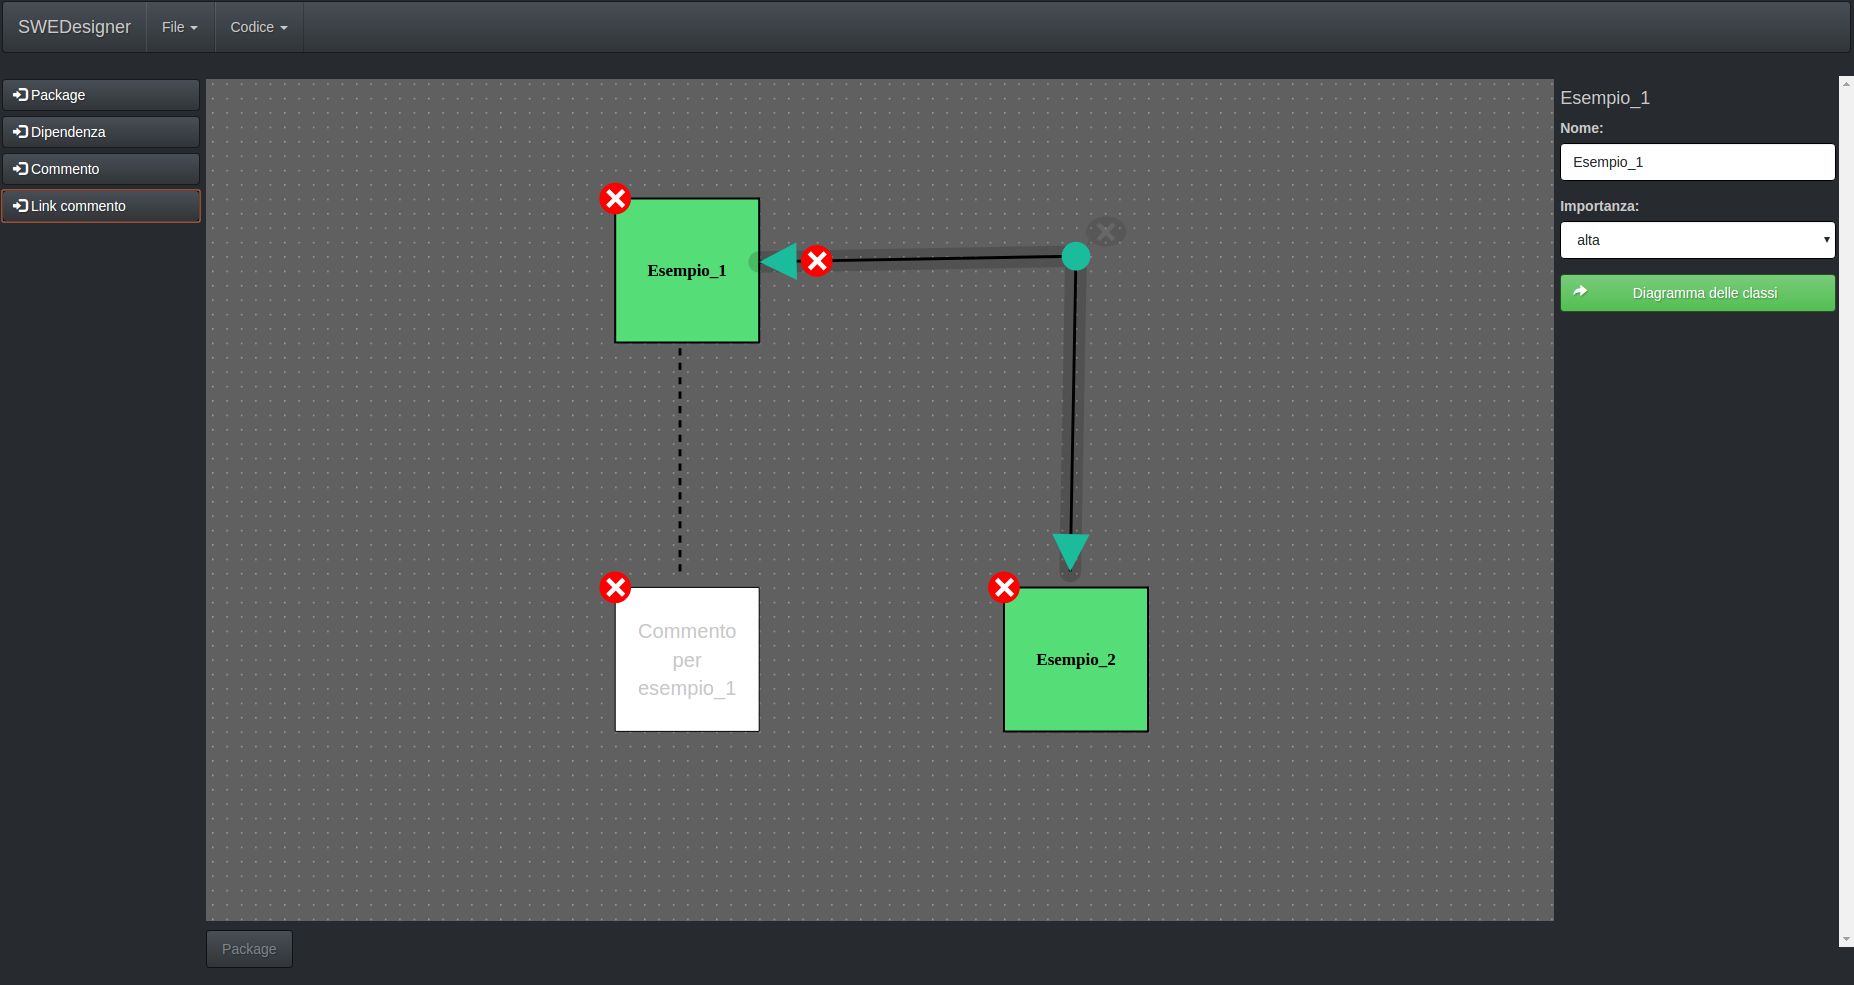
\includegraphics[scale=0.24]{./Immagini/PackageDiagram.png}
				\caption{Editor del diagramma dei package}\label{fig:PackageDiagram}
			\end{figure}
		\newpage
		\subsection{Editor del diagramma delle classi}
			Nel diagramma delle classi è possibile gestire l'architettura delle componenti del package di
			appartenenza.
			\subsubsection{Menù degli strumenti}
				Sono messi a disposizione i seguenti strumenti per editare il diagramma delle classi:
				\begin{itemize}
					\item \textit{\textbf{Classe}}: cliccare il pulsante e poi cliccare il luogo desiderato
					dell'area di lavoro per crearvi una classe;
					\item \textit{\textbf{Interfaccia}}: cliccare il pulsante e poi cliccare il luogo desiderato
					dell'area di lavoro per crearvi un'interfaccia;
					\item \textit{\textbf{Generalizzazione}}: cliccare il pulsante, cliccare l'elemento sorgente
					e successivamente quello destinatario per creare una relazione di generalizzazione;
					\item \textit{\textbf{Implementazione}}: cliccare il pulsante, cliccare l'elemento sorgente
					e successivamente quello destinatario per creare una relazione di implementazione;
					\item \textit{\textbf{Aggregazione}}: cliccare il pulsante, cliccare l'elemento sorgente
					e successivamente quello destinatario per creare una relazione di aggregazione;
					\item \textit{\textbf{Composizione}}: cliccare il pulsante, cliccare l'elemento sorgente
					e successivamente quello destinatario per creare una relazione di composizione;
					\item \textit{\textbf{Associazione}}: cliccare il pulsante, cliccare l'elemento sorgente
					e successivamente quello destinatario per creare una relazione di associazione;
					\item \textit{\textbf{Commento}}: cliccare il pulsante e poi cliccare il luogo desiderato
					dell'area di lavoro per crearvi un commento;
					\item \textit{\textbf{Link commento}}: cliccare il pulsante, cliccare l'elemento ed il
					commento desiderati per collegarli.
				\end{itemize}
				Per spostare un elemento (Classe, Interfaccia o Commento) all'interno dell'area di lavoro,
				cliccarlo con il mouse e trascinarlo verso la posizione desiderata.\\
				Per cambiare un membro di una relazione, trascinarne un apice sull'elemento
				desiderato.\\
				Per "spezzare" una relazione in un punto specifico della linea, eseguire un doppio click sulla
				posizione desiderata.\\
				Per eliminare un elemento dal diagramma, cliccare sulla rispettiva icona nell'area di lavoro
				avente una croce rossa.
			\subsubsection{Pannello delle proprietà}
				Cliccando su un elemento del diagramma delle classi verrà visualizzato il corrispondente pannello
				di dettaglio contenente tutte le proprietà modificabili dell'elemento stesso.\\
				Per modificare una proprietà testuale, editare il campo di testo e successivamente premere il
				tasto "Invio" della tastiera oppure cliccare altrove nell'applicazione.\\
				Per modificare una proprietà non testuale, cambiare semplicemente il valore selezionando quello
				desiderato.\\
				Per aggiungere un attributo\footnote{Funzionalità disponibile solo per elementi Classe.},
				selezionare il pulsante \textit{\textbf{Attributi}} ed il pulsante \textit{\textbf{+ Attributo}}.
				Per aggiungere un'operazione\footnote{Funzionalità disponibile per elementi Classe ed Interfaccia.},
				selezionare il pulsante \textit{\textbf{Operazioni}} ed il pulsante \textit{\textbf{+ Operazione}}.
				Nel pannello proprietà di classi e interfacce, per ogni sotto-pannello di operazione definita,
				è possibile spostarsi al rispettivo diagramma delle bubble premendo il relativo pulsante
				\textit{\textbf{BubbleDiagram}}.
			\begin{figure} [h!]
				\centering
				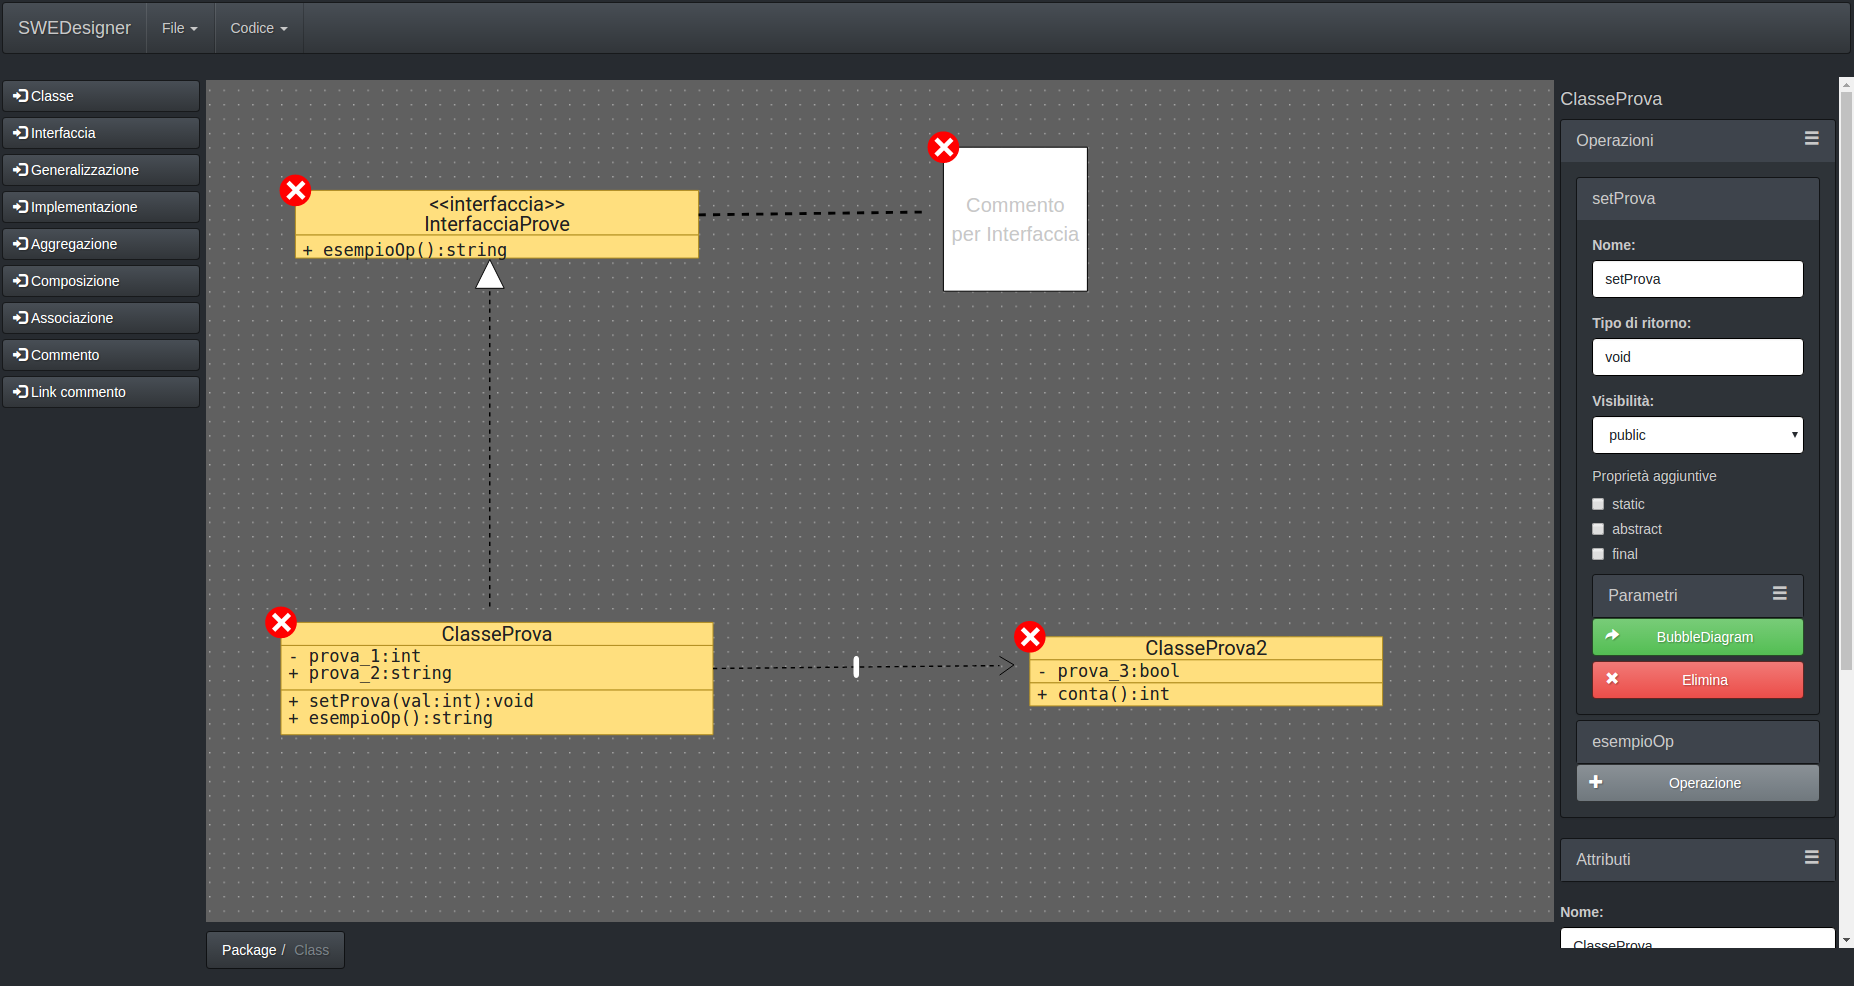
\includegraphics[scale=0.24]{./Immagini/ClassDiagram.png}
				\caption{Editor del diagramma delle classi}\label{fig:ClassDiagram}
			\end{figure}
		\newpage
		\subsection{Editor del diagramma delle bubble}\label{sez:BubbleDiagram}
			Nel diagramma delle bubble è possibile strutturare ed ordinare i passi da compiere di un'operazione
			facente parte di una classe o interfaccia definita.
			Questo tipo di diagramma è stato ideato e dal team di sviluppo di \progetto\
			e si discosta dai diagrammi UML di attività e sequenza. Tende piuttosto ad assomigliare ad un
			flow-chart.\\
			Una bubble è un elemento del diagramma e rispecchia una determinata istruzione (o set di
			istruzioni) traducibili in codice sorgente (condizione, ciclo, ...).\\
			È possibile realizzare set di istruzioni definite da bubble innestandole tra loro\footnote{Maggiori informazioni alla definizione dello strumento \textit{\textbf{Innesta}}, nella sezione \ref{sez:BubbleDiagram-strumenti}}.
			Ogni diagramma delle bubble è caratterizzato da una bubble \textit{\textbf{Start}} che segna
			il punto d'inizio dell'operazione
			\subsubsection{Menù degli strumenti}\label{sez:BubbleDiagram-strumenti}
				Le diverse bubble inseribili nel diagramma sono:
				\begin{itemize}
					\item \textit{\textbf{Start}}: specifica il punto di inizio dell'algoritmo che si sta
					sviluppando. Deve essere inserita anche per indicare il punto iniziale di un blocco di bubble
					innestate tra loro (vedi fig. \ref{fig:BubbleDiagram}).\\
					Per crearla, cliccare il pulsante e poi cliccare il luogo desiderato
					dell'area di lavoro;
					\item \textit{\textbf{Custom}}: al suo interno, l'utente può definire un insieme di istruzioni
					(dallo specifico pannello delle proprietà) che saranno copiate nel codice sorgente generato.\\
					Per crearla, cliccare il pulsante e poi cliccare il luogo desiderato
					dell'area di lavoro;
					\item \textit{\textbf{If}}: corrisponde all'istruzione condizionale ``if''; specifica un blocco
					di bubble (da innestare) eseguibili al verificarsi di una condizione.\\
					Per crearla, cliccare il pulsante e poi cliccare il luogo desiderato
					dell'area di lavoro;
					\item \textit{\textbf{Else}}: corrisponde all'istruzione condizionale ``else''; specifica un
					blocco di bubble (da innestare) eseguibili alternativamente al non	verificarsi di una
					condizione.\\
					Per crearla, cliccare il pulsante e poi cliccare il luogo desiderato
					dell'area di lavoro;
					\item \textit{\textbf{For}}: corrisponde all'istruzione iterativa ``for''; specifica un
					blocco di bubble (da innestare) la cui esecuzione verrà ripetuta fino al verificarsi della
					condizione impostata.\\
					Per crearla, cliccare il pulsante e poi cliccare il luogo desiderato
					dell'area di lavoro;
					\item \textit{\textbf{Return}}: corrisponde all'istruzione ``return''; definisce la variabile
					o un valore da ritornare.\\
					Per crearla, cliccare il pulsante e poi cliccare il luogo desiderato
					dell'area di lavoro;
					\item \textit{\textbf{While}}: specifica un blocco di bubble (da innestare) la cui esecuzione
					verrà ripetuta fino al verificarsi della condizione impostata.\\
					Per crearla, cliccare il pulsante e poi cliccare il luogo desiderato
					dell'area di lavoro;
					\item \textit{\textbf{Link}}: specifica l'ordine di esecuzione tra due bubble.\\
					Per crearla, cliccare il pulsante, cliccare l'elemento antecedente
					e successivamente quello successivo per creare una relazione di esecuzione sequenziale;
					\item \textit{\textbf{Innesta}}: utilizzabile per innestare una bubble dentro l'altra.
					In un concetto di semplice esecuzione dell'operazione in sviluppo, la
					logica della struttura del codice di bubble innestate è la seguente:
					\begin{enumerate}
						\item Prima viene eseguito il codice definito nella bubble innestante (ad esempio,
						condizione ``if``, controllo di ciclo ``while'', ...);
						\item All'interno del blocco definito nella bubble innestante viene eseguito il codice
						definito sequenzialmente a partire dalla bubble \textit{\textbf{Start}}.
					\end{enumerate}
					È possibile effettuare molteplici annidamenti.\\
					Per innestare, cliccare il pulsante, cliccare la specifica bubble
					e successivamente la bubble contenitrice;
				\end{itemize}
				Per spostare una bubble all'interno dell'area di lavoro,
				cliccarla con il mouse e trascinarla verso la posizione desiderata.\\
				Per cambiare un membro di una relazione, trascinarne un apice sull'elemento
				desiderato.\\
				Per "spezzare" una relazione in un punto specifico della linea, eseguire un doppio click sulla
				posizione desiderata.\\
				Per eliminare un elemento dal diagramma, cliccare sulla rispettiva icona nell'area di lavoro
				avente una croce rossa.
			\subsubsection{Pannello delle proprietà}
				Cliccando su un elemento del diagramma delle classi verrà visualizzato il corrispondente pannello
				di dettaglio contenente tutte le proprietà modificabili dell'elemento stesso.\\
				Per modificare una proprietà testuale, editare il campo di testo e successivamente premere il
				tasto "Invio" della tastiera oppure cliccare altrove nell'applicazione. Per le bubble \textit{\textbf{Custom}}, una volta terminato di inserire il codice nell'apposito spazio, premere il pulsante \textit{\textbf{Salva codice}}.\\
				Per modificare una proprietà non testuale, cambiare semplicemente il valore selezionando quello
				desiderato.\\
				Per riconoscere più facilmente il significato di una bubble all'interno del grafo, è possibile
				assegnarvi un commento dal relativo pannello delle proprietà (campo ``Commento'').
			\begin{figure} [h!]
				\centering
				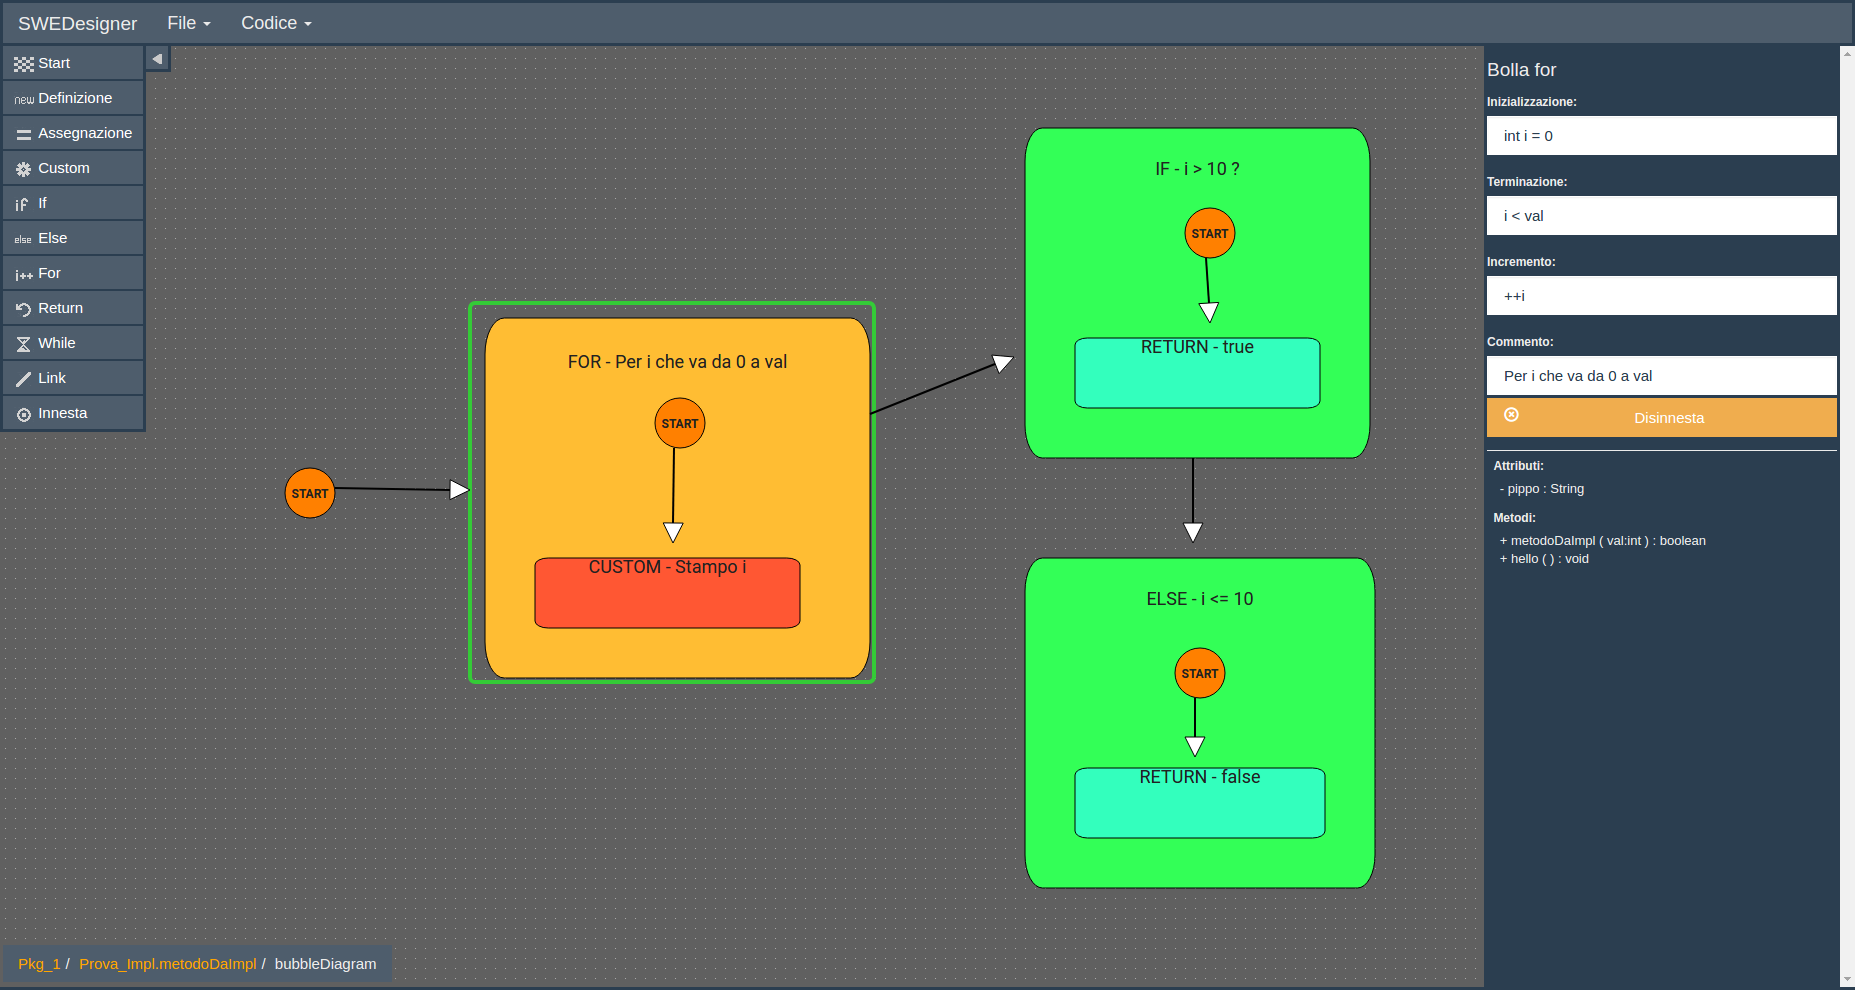
\includegraphics[scale=0.24]{./Immagini/BubbleDiagram.png}
				\caption{Editor del diagramma delle bubble}\label{fig:BubbleDiagram}
			\end{figure}
\end{document}
